\documentclass[17pt,a4paper,landscape]{extarticle}
\usepackage[margin=2.35cm,top=0.12cm,left=1.05cm]{geometry}
\usepackage{amsmath}
\usepackage{amssymb}
\usepackage{tasks}
\usepackage{tikz}
\usepackage{xcolor}
\usepackage[sfdefault,lf]{FiraSans}
\renewcommand{\familydefault}{\sfdefault}
\setlength{\parindent}{0pt}
\pagestyle{empty}
\settasks{label=\textbf{\arabic*.}, label-width=2.2em, item-indent=2.95em, column-sep=2.1cm, after-item-skip=5.1em}
\renewcommand{\arraystretch}{1.15}
\everymath{\displaystyle}

\newcommand{\twocointree}{%
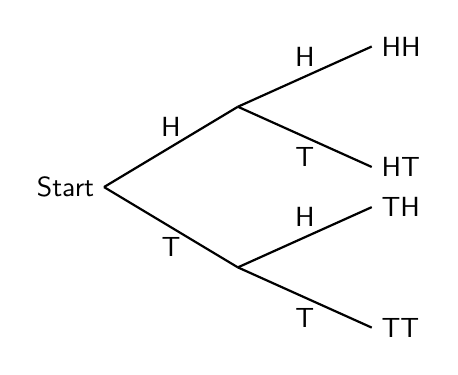
\begin{tikzpicture}[x=0.85cm,y=0.85cm]
  \draw[thick] (0,0) -- (2,1.2) node[midway,above] {H};
  \draw[thick] (0,0) -- (2,-1.2) node[midway,below] {T};
  \draw[thick] (2,1.2) -- (4,2.1) node[midway,above] {H};
  \draw[thick] (2,1.2) -- (4,0.3) node[midway,below] {T};
  \draw[thick] (2,-1.2) -- (4,-0.3) node[midway,above] {H};
  \draw[thick] (2,-1.2) -- (4,-2.1) node[midway,below] {T};
  \node[left] at (0,0) {Start};
  \node[right] at (4,2.1) {HH};
  \node[right] at (4,0.3) {HT};
  \node[right] at (4,-0.3) {TH};
  \node[right] at (4,-2.1) {TT};
\end{tikzpicture}%
}

\newcommand{\coindietree}{%
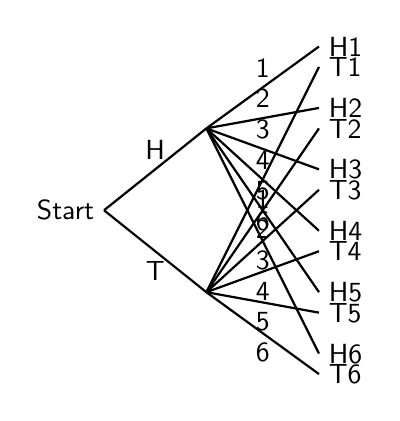
\begin{tikzpicture}[x=0.65cm,y=0.65cm]
  \draw[thick] (0,0) -- (2,1.6) node[midway,above] {H};
  \draw[thick] (0,0) -- (2,-1.6) node[midway,below] {T};
  \foreach \y/\n/\lab in {3.2/1/H1,2.0/2/H2,0.8/3/H3,-0.4/4/H4,-1.6/5/H5,-2.8/6/H6} {
    \draw[thick] (2,1.6) -- (4.2,\y) node[midway,above] {\n};
    \node[right] at (4.2,\y) {\lab};
  }
  \foreach \y/\n/\lab in {2.8/1/T1,1.6/2/T2,0.4/3/T3,-0.8/4/T4,-2.0/5/T5,-3.2/6/T6} {
    \draw[thick] (2,-1.6) -- (4.2,\y) node[midway,below] {\n};
    \node[right] at (4.2,\y) {\lab};
  }
  \node[left] at (0,0) {Start};
\end{tikzpicture}%
}


\begin{document}
\sffamily
\boldmath

\vspace*{0.4em}
{\LARGE \textbf{Foundation}}
\begin{tasks}(2)
\task {Use this tree to list the possible outcomes for two fair coin tosses.

\vspace{0.4em}\twocointree}
\task {Use the tree to say how many outcomes are possible when two fair coins are tossed.

\vspace{0.4em}\twocointree}
\task {Use the tree to write the probability of getting HH.

\vspace{0.4em}\twocointree}
\task {Use the tree to write the probability of getting TT.

\vspace{0.4em}\twocointree}
\task {Use the tree to write the probability of getting exactly one head.

\vspace{0.4em}\twocointree}
\task {Use this tree for a coin toss and a fair die roll. How many outcomes are possible altogether?

\vspace{0.4em}\coindietree}
\task {Use the tree to find the probability of getting H and $3$.

\vspace{0.4em}\coindietree}
\task {Use the tree to find the probability of getting T and an even number.

\vspace{0.4em}\coindietree}
\task {Fill in the blank using the coin tree: the probability of at least one tail is $\frac{\square}{4}$.}
\task {Fill in the blank using the coin-and-die tree: the probability of heads is $\frac{\square}{12}$.}
\task {Which is more likely when two fair coins are tossed: two heads or exactly one head?}
\task {A student says there are only three outcomes when two coins are tossed: heads, tails, and one of each. Are they correct?}
\end{tasks}

\end{document}
